\documentclass[landscape]{exam}
\usepackage{2in1, lscape} 

\usepackage{units} 
\usepackage{parskip} 
\usepackage{xfrac} 
\usepackage[fleqn]{amsmath}
\usepackage{commath}
\usepackage{cancel}
\usepackage{float}
\usepackage{mdwlist}
\usepackage{booktabs}
\usepackage{cancel}
\usepackage{polynom}
\usepackage{caption}
\usepackage{fullpage}
\usepackage{comment}
\usepackage{enumerate}
\usepackage{graphicx}
\usepackage{mathtools} 

\newcommand{\degree}{\ensuremath{^\circ}} 
\everymath{\displaystyle}

% \begin{figure}[H]
%   \centering
%   \includegraphics[scale=.3]{problem7.eps}
%   \caption*{Problem 7}
% \end{figure}

% \begin{tabular}{cc}
% \toprule
% period & amplitude \\
% \midrule
%   $\pi$ & $2$ \\
% \bottomrule
% \end{tabular}

\printanswers{}

\ifprintanswers{}
  \usepackage{2in1, lscape} 
\fi

\date{\today}
\author{}
\title{Math 141 \\ Homework 7}

\begin{document}

\maketitle

\section{Homework}

\begin{itemize*}
  \item Read Section 3.1
  \item Section 3.1: 5--17, 21, 23--30, 33, 35--36
\end{itemize*}

\ifprintanswers{}
  \pagebreak
\fi

\section{Extra Credit}
Section 3.1: 73

\ifprintanswers{}

  If $f(x)$ is a monomial with $x$ raised to an even power, then $f(x)$ is an even function.  If $n$ is a positive
  integer:
  \begin{align*}
    f(x)  &= x^{2n} \\
    \\
    f(-x) &= \del{ -x }^{2n} \\
          &= x^{2n} \\
          &= f(x) \\
  \end{align*}

  If $f(x)$ is a monomial with $x$ raised to an odd power, then $f(x)$ is an odd function
  \begin{align*}
    f(x)  &= x^{2n + 1} \\
    \\
    f(-x) &= \del{ -x }^{2n + 1} \\
          &= \del{ -x }^{2n} (-x) \\
          &= x^{2n} (-x) \\
          &= -x^{2n + 1} \\
          &= -f(x) \\
  \end{align*}

  If you add two even functions, you get another even function.  If $f$ and $g$ are both even, then $f(-x) = f(x)$ and
  $g(-x) = g(x)$ and
  \begin{align*}
    (f + g)(-x) &= f(-x) + g(-x) \\
                &= f(x) + g(x) \\
                &= (f + g)(x) \\
  \end{align*}

  If you add two odd functions, you get another odd function.  If $f$ and $g$ are both odd, then $f(-x) = -f(x)$ and
  $g(-x) = -g(x)$ and
  \begin{align*}
    (f + g)(-x) &= -f(x) - g(x) \\
                &= -(f(x) + g(x)) \\
                &= - (f + g)(x) \\
  \end{align*}

  If you add an even and odd function, the new function is neither odd nor even.  If $f$ is even and $g$ is odd, then
  $f(-x) = f(x)$ and $g(-x) = -g(x)$ and
  \begin{align*}
    (f + g)(-x) &= f(x) - g(x) \\
                &\neq (f + g)(x) \\
                &\neq -(f + g)(x) \\
  \end{align*}

  Now we've proven all the facts needed for the problem.

  \begin{enumerate}[a]
    \item If a polynomial contains only odd powers, it is a sum of odd functions so it is also an odd function.

    \item If a polynomial contains only even powers, it is a sum of even functions so it is also an even function.

    \item If a polynomial contains both even and odd powers, it is a sum of even and odd functions so it is neither even
      nor odd.

    \item
      \begin{align*}
        f(x) &= -x^2 + 5 \\
        g(x) &= x^5 + 6x^3 - 2x \\
      \end{align*}

  \end{enumerate}

%  Here's a graph of all three functions:
%  \begin{figure}[H]
%    \centering
%    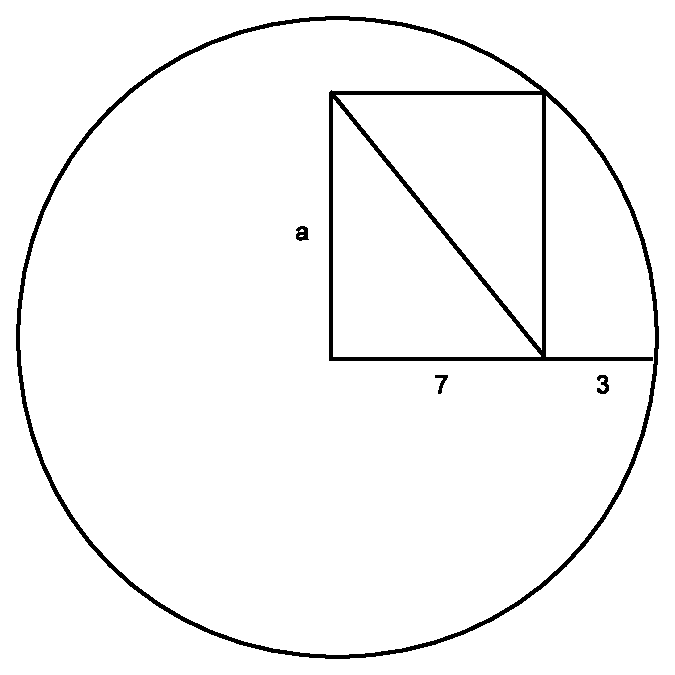
\includegraphics{extra-credit.eps}
%    \caption{Extra Credit}
%  \end{figure}

  \ifprintanswers{}
    \pagebreak
  \fi

  \section{Review}
  \begin{enumerate}
    \item Find the domain: $f(x) = \frac{1}{\sqrt{x^2 - x - 20}}$
      \begin{solution}
        \begin{align*}
          x^2 - x - 20   &> 0 \\
          (x - 5)(x + 4) &> 0 \\
          \\
          x &= \left( -\infty, -4 \right) \cup \left( 5, \infty \right) \\
        \end{align*}
      \end{solution}

    \item Find the domain: $f(x) = \sqrt{4 - x^2}$
      \begin{solution}
        \begin{align*}
          4 - x^2 &> 0 \\
          (2 - x)(2 + x) &> 0 \\
          \\
          x &= [-2, 2] \\
        \end{align*}
      \end{solution}

    \item $f(x) = x^2 + 3x$ 
      \begin{enumerate}[a]
        \item Put in standard form.
          \begin{solution}
            \begin{align*}
              f(x) &= x^2 + 3x \\
              &= x^2 + 3x + \frac{9}{4} - \frac{9}{4} \\
              &= \del{ x + \frac{3}{2} }^2 - \frac{9}{4} \\
            \end{align*}
          \end{solution}

        \item Find the vertex.
          \begin{solution}
            $ \left( -\frac{3}{2}, - \frac{9}{4} \right) $
          \end{solution}

      \end{enumerate}

    \item $f(x) = 2x^2 + 4x$ 
      \begin{enumerate}[a]
        \item Put in standard form.
          \begin{solution}
            \begin{align*}
              f(x)           &= 2x^2 + 4x \\
              \frac{f(x)}{2} &= x^2 + 2x \\
                             &= x^2 + 2x + 1 - 1 \\
                             &= \del{x + 1}^2 - 1 \\
              f(x)           &= 2\del{x + 1}^2 - 2 \\
            \end{align*}
          \end{solution}
        \item Find the vertex.
          \begin{solution}
            $ (-1, -2) $
          \end{solution}

      \end{enumerate}

  \end{enumerate}

  \pagebreak

  \section{Section 3.1}

  \begin{description}

    \item[5] III---odd power with positive leading coefficient

    \item[6] I---even power with negative leading coefficient

    \item[7] V---odd power with negative leading coefficient
      
    \item[8] II---even power with positive leading coefficient, not shrunk vertically
      
    \item[9] VI---even power with positive leading coefficient, shrunk vertically

    \item[10] IV---odd power with negative leading coefficient

    \item[11]
      \begin{figure}[H]
        \centering
        \includegraphics[scale=0.9]{problem11.eps}
        \caption*{Problem 11: $P(x) = (x - 1)(x + 2)$}
      \end{figure}

    \item[12]
      \begin{figure}[H]
        \centering
        \includegraphics[scale=0.9]{problem12.eps}
        \caption*{Problem 12: $P(x) = (x - 1)(x + 1)(x - 2)$}
      \end{figure}

    \item[13]
      \begin{figure}[H]
        \centering
        \includegraphics[scale=0.9]{problem13.eps}
        \caption*{Problem 13: $P(x) = x(x - 3)(x + 2)$}
      \end{figure}

    \item[14]
      \begin{figure}[H]
        \centering
        \includegraphics[scale=0.9]{problem14.eps}
        \caption*{Problem 14: $P(x) = (2x - 1)(x + 1)(x + 3)$}
      \end{figure}

    \item[15]
      \begin{figure}[H]
        \centering
        \includegraphics[scale=0.9]{problem15.eps}
        \caption*{Problem 15: $P(x) = (x - 3)(x + 2)(3x - 2)$}
      \end{figure}

    \item[16]
      \begin{figure}[H]
        \centering
        \includegraphics[scale=0.9]{problem16.eps}
        \caption*{Problem 16: $P(x) = \frac{1}{5} x \del{x - 5}^2$}
      \end{figure}

    \item[17]
      \begin{figure}[H]
        \centering
        \includegraphics[scale=0.9]{problem17.eps}
        \caption*{Problem 17: $P(x) = \del{x - 1}^2(x - 3)$}
      \end{figure}

    \item[21]
      \begin{figure}[H]
        \centering
        \includegraphics[scale=0.9]{problem21.eps}
        \caption*{Problem 21: $P(x) = x^3(x + 2)\del{x - 3}^2$}
      \end{figure}

    \item[23] 
      \begin{align*}
        P(x) &= x^3 - x^2 - 6x \\
             &= x(x^2 - x - 6) \\
             &= x(x + 2)(x - 3) \\
        x    &= \{ -2, 0, 3 \} \\
      \end{align*}
      
      \begin{figure}[H]
        \centering
        \includegraphics[scale=0.9]{problem23.eps}
        \caption*{Problem 23}
      \end{figure}

    \item[24] 
      \begin{align*}
        P(x) &= x^3 + 2x^2 - 8x \\
             &= x(x^2 + 2x - 8) \\
             &= x(x + 4)(x - 2) \\
        x    &= \{ -4, 0, 2 \} \\
      \end{align*}
      
      \begin{figure}[H]
        \centering
        \includegraphics[scale=0.9]{problem24.eps}
        \caption*{Problem 24}
      \end{figure}

    \item[25] 
      \begin{align*}
        P(x) &= -x^3 + x^2 + 12x \\
             &= -x(x^2 - x - 12) \\
             &= -x(x - 4)(x + 3) \\
        x    &= \{ -3, 0, 4 \} \\
      \end{align*}
      
      \begin{figure}[H]
        \centering
        \includegraphics[scale=0.9]{problem25.eps}
        \caption*{Problem 25}
      \end{figure}

    \item[26] 
      \begin{align*}
        P(x) &= -2x^3 - x^2 - x \\
             &= -x(2x^2 - x - 1) \\
             &= -x(2x - 1)(x + 1) \\
        x    &= \left\{ -1, 0, \frac{1}{2} \right\} \\
      \end{align*}
      
      \begin{figure}[H]
        \centering
        \includegraphics[scale=0.9]{problem26.eps}
        \caption*{Problem 26}
      \end{figure}

    \item[27] 
      \begin{align*}
        P(x) &= x^4 - 3x^3 + 2x^2 \\
             &= x^2(x^2 - 3x + 2) \\
             &= x^2(x - 1)(x - 2) \\
        x    &= \{ 0, 1, 2 \} \\
      \end{align*}
      
      \begin{figure}[H]
        \centering
        \includegraphics[scale=0.9]{problem27.eps}
        \caption*{Problem 27}
      \end{figure}

    \pagebreak

    \item[28] 
      \begin{align*}
        P(x) &= x^5 - 9x^3 \\
             &= x^3(x^2 - 9) \\
             &= x^3(x - 3)(x + 3) \\
        x    &= \{ -3, 0, 3 \} \\
      \end{align*}
      
      \begin{figure}[H]
        \centering
        \includegraphics[scale=0.9]{problem28.eps}
        \caption*{Problem 28}
      \end{figure}

    \pagebreak

    \item[29] 
      \begin{align*}
        P(x) &= x^3 + x^2 - x - 1 \\
             &= x^2(x + 1) - (x + 1) \\
             &= (x^2 - 1)(x + 1) \\
             &= (x - 1)(x + 1)(x + 1) \\
             &= (x - 1)\del{x + 1}^2 \\
        x    &= \{ -1, 1 \} \\
      \end{align*}
      
      \begin{figure}[H]
        \centering
        \includegraphics[scale=0.9]{problem29.eps}
        \caption*{Problem 29}
      \end{figure}

    \pagebreak

    \item[30] 
      \begin{align*}
        P(x) &= x^3 + 3x^2 - 4x - 12 \\
             &= x^2(x + 3) - 4(x + 3) \\
             &= (x^2 - 4)(x + 3) \\
             &= (x - 2)(x + 2)(x + 3) \\
        x    &= \{ -3, -2, 2 \} \\
      \end{align*}
      
      \begin{figure}[H]
        \centering
        \includegraphics[scale=0.9]{problem30.eps}
        \caption*{Problem 30}
      \end{figure}

    \pagebreak

    \item[33] 
      \begin{align*}
        P(x) &= x^4 - 2x^3 - 8x + 16 \\
             &= x^3(x - 2) - 8(x - 2) \\
             &= (x^3 - 8)(x - 2) \\
             &= (x - 2)(x - 2)(x^2 + 2x + 4) \text{ difference of two cubes} \\
             &= \del{x - 2}^2(x^2 + 2x + 4) \\
        x    &= 2 \\
      \end{align*}
      
      \begin{figure}[H]
        \centering
        \includegraphics[scale=0.9]{problem33.eps}
        \caption*{Problem 33}
      \end{figure}

    \item[35] 
      \begin{align*}
        P(x) &= x^4 - 3x^2 - 4 \\
             &= (x^2 - 4)(x^2 + 1) \\
             &= (x - 2)(x + 2)(x^2 + 1) \\
        x    &= \{-2, 2 \} \\
      \end{align*}
      
      \begin{figure}[H]
        \centering
        \includegraphics[scale=0.9]{problem35.eps}
        \caption*{Problem 35}
      \end{figure}

    \item[36] 
      \begin{align*}
        P(x) &= x^6 - 2x^3 + 1 \\
             &= \del{x^3 - 1}^2 \\
             &= \del{(x - 1)(x^2 + x + 1)}^2 \\
             &= \del{x - 1}^2 \del{x^2 + x + 1}^2 \\
        x    &= 1 \\
      \end{align*}
      
      \begin{figure}[H]
        \centering
        \includegraphics[scale=0.9]{problem36.eps}
        \caption*{Problem 36}
      \end{figure}

  \end{description}
\else
  \vspace{9 cm}
  \begin{quote}
    \begin{em}
      A good person will resist an evil system with his whole soul. Disobedience of the laws of an evil state is
      therefore a duty.
    \end{em}
  \end{quote}
  \hspace{1 cm} --Mahatma Gandhi

\fi

\end{document}

